\chapter{Les plantes autour de nous}\label{ch:g1:plants-around-us}

Une pâquerette dans la pelouse, de la mousse sur le mur, le grand
marronnier de la cour~: aucun d'eux ne s'enfuira jamais, et pourtant
tous sont vivants. Les \omterm{def:g1:plants-around-us:plant}{plantes} sont les \omterm{def:g1:living-or-not:living}{êtres vivants} tranquilles
--- elles naissent, se nourrissent, grandissent, parfois pendant des
centaines d'années, sans jamais bouger de leur place.

\section{Les plantes sont des êtres vivants}

\begin{definition}[Plante]\label{def:g1:plants-around-us:plant}
Une \emph{plante}\index{plante} est un \omterm{def:g1:living-or-not:living}{être vivant} qui reste fixé
dans le sol et qui fabrique lui-même sa nourriture, grâce à la
lumière. L'herbe, les pâquerettes, les pieds de tomate et les \omterm{def:g1:plants-around-us:tree}{arbres}
sont tous des plantes. La plupart des plantes sont vertes.
\end{definition}

\begin{example}[La pâquerette est vivante]\label{ex:g1:plants-around-us:daisy}
Vérifie les signes de la vie sur une pâquerette~: elle est née d'une
graine~; elle se nourrit --- d'eau prise dans le sol et de lumière
venue du ciel~; elle grandit~; elle fait des graines qui deviennent
de nouvelles pâquerettes~; elle meurt au gel. Tous les signes sont
là. La pâquerette est aussi vivante que le chat --- elle est
simplement bien plus discrète.
\end{example}

\begin{omfigure}
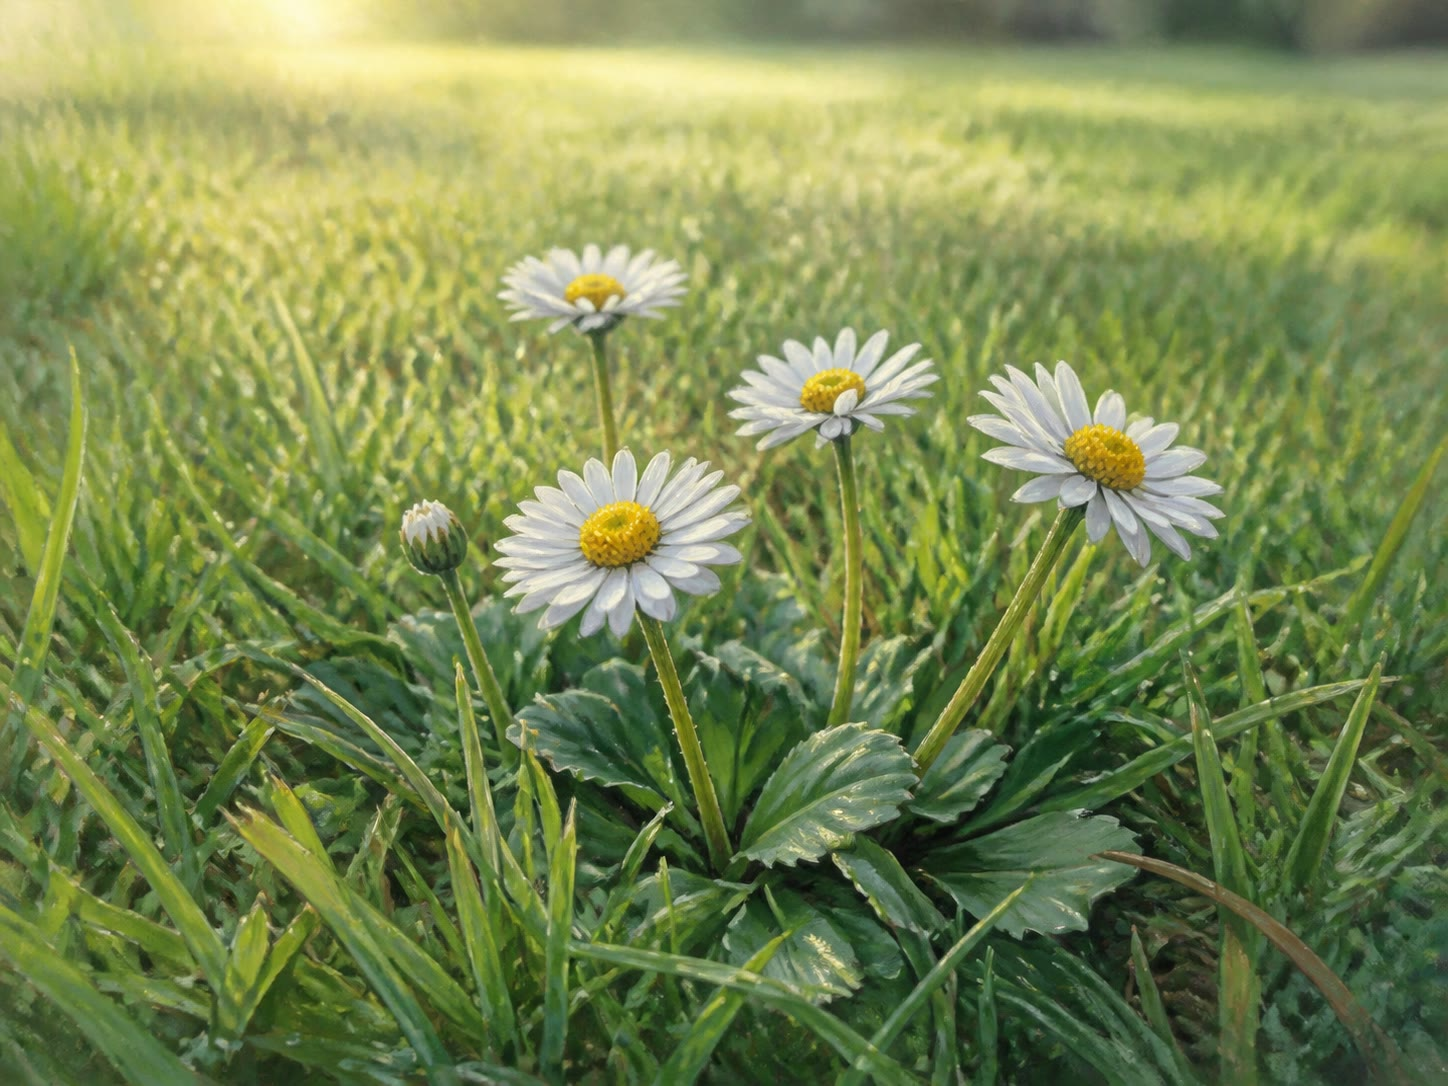
\includegraphics[width=0.58\linewidth]{images/book1/ai/g1-plants-daisy.jpg}

{\small Des pâquerettes dans la pelouse~: nées de graines, nourries
de lumière et d'eau, vivantes en silence.}
\end{omfigure}

\begin{remark}[Vivant sans courir]\label{rem:g1:plants-around-us:still}
Les \omterm{def:g1:plants-around-us:plant}{plantes} ne marchent pas, mais elles ne sont pas tout à fait
immobiles. Un tournesol se tourne pour suivre la lumière au fil de
la journée, et une \omterm{def:g1:plants-around-us:plant}{plante} posée sur un rebord de fenêtre penche
lentement vers la vitre. Les \omterm{def:g1:plants-around-us:plant}{plantes} se déplacent en
\emph{grandissant} --- trop lentement pour nos yeux, assez vite pour
une semaine d'observation.
\end{remark}

\section{Les parties d'une plante}

\begin{definition}[Les parties d'une plante]\label{def:g1:plants-around-us:parts}
Une \omterm{def:g1:plants-around-us:plant}{plante} à fleurs a quatre parties principales~:
\begin{enumerate}
  \item les \emph{racines}\index{racine}, cachées dans le sol, qui
        tiennent la \omterm{def:g1:plants-around-us:plant}{plante} en place et boivent l'eau~;
  \item la \emph{tige}\index{tige}, qui dresse la \omterm{def:g1:plants-around-us:plant}{plante} et porte
        l'eau jusqu'aux feuilles~;
  \item les \emph{feuilles}\index{feuille}, plates et vertes, qui
        attrapent la lumière~;
  \item la \emph{fleur}\index{fleur}, qui fera les graines.
\end{enumerate}
\end{definition}

\begin{omfigure}
\begin{tikzpicture}
  \node[anchor=south west, inner sep=0] (img) at (0,0)
    {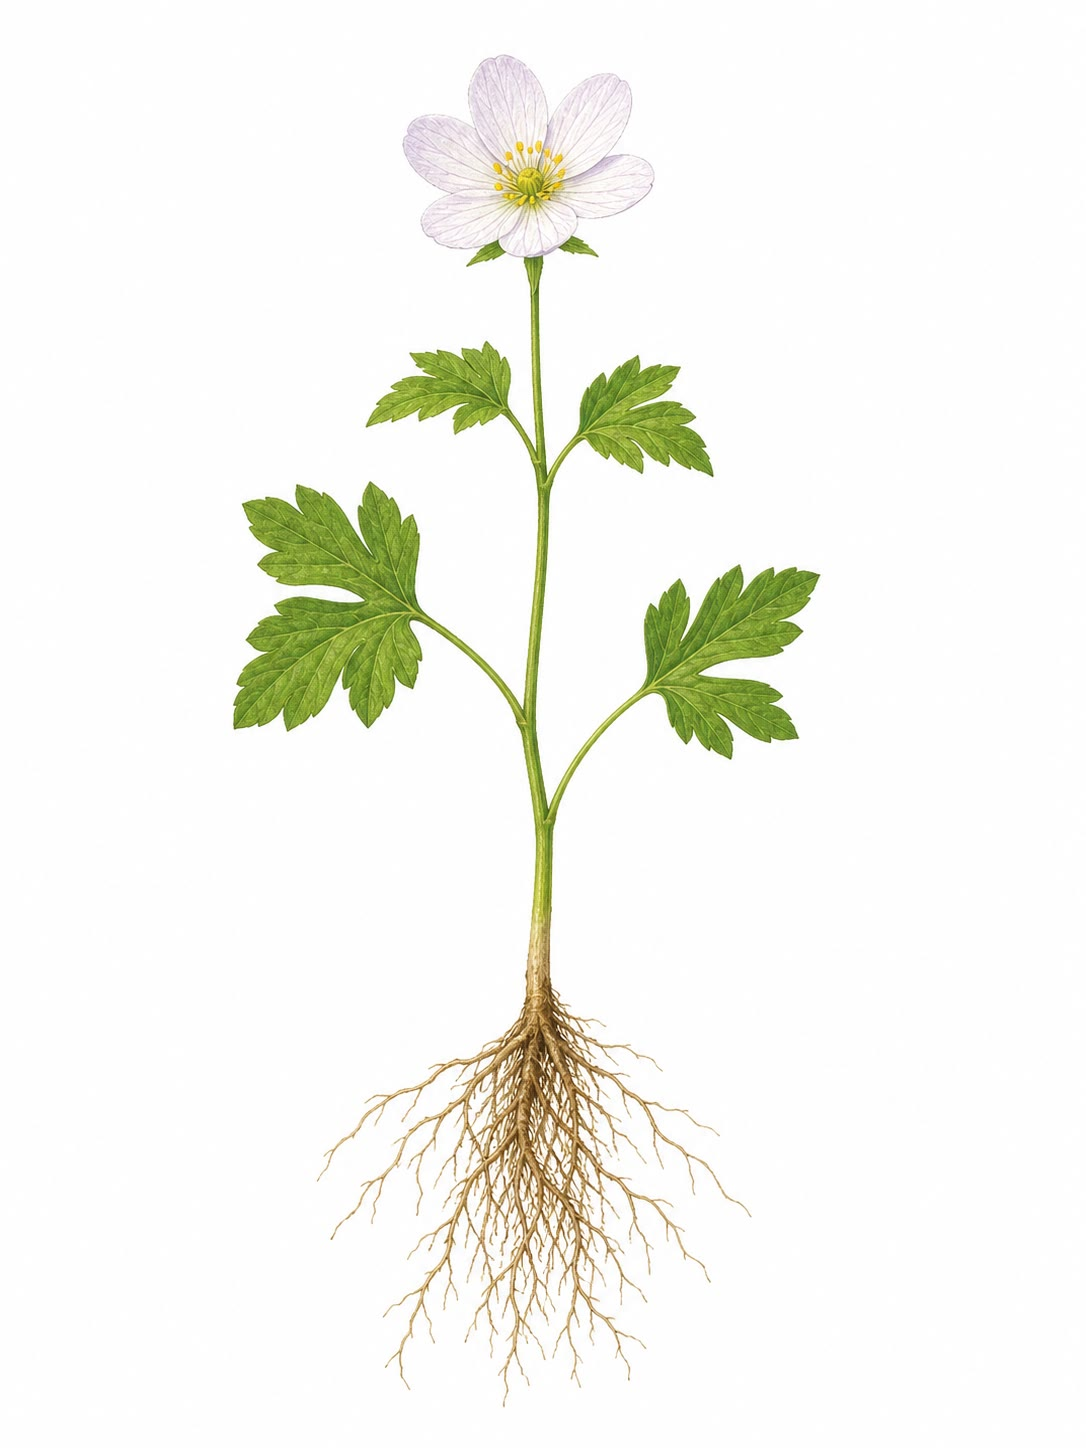
\includegraphics[width=0.5\linewidth]{images/book1/ai/fig-plant-uprooted.jpg}};
  \begin{scope}[x={(img.south east)}, y={(img.north west)},
      every node/.style={font=\small}]
    \draw[omDef, thick] (0.55,0.91) -- (0.74,0.93) node[right] {fleur};
    \draw[omDef, thick] (0.68,0.57) -- (0.84,0.62) node[right] {feuille};
    \draw[omDef, thick] (0.51,0.33) -- (0.74,0.36) node[right] {tige};
    \draw[omDef, thick] (0.58,0.13) -- (0.78,0.16) node[right] {racines};
  \end{scope}
\end{tikzpicture}

{\small Les quatre parties d'une \omterm{def:g1:plants-around-us:plant}{plante} à \omterm{def:g1:plants-around-us:parts}{fleurs}, montrée arrachée
tout entière~: dans la terre, les \omterm{def:g1:plants-around-us:parts}{racines} font leur travail à
l'abri des regards, sous le sol.}
\end{omfigure}

\begin{example}[Arracher une mauvaise herbe]\label{ex:g1:plants-around-us:weed}
Arrache doucement une mauvaise herbe d'une terre meuble et humide,
et tu remontes la partie cachée~: une touffe de \omterm{def:g1:plants-around-us:parts}{racines} pâles,
parfois plus longue que toute la \omterm{def:g1:plants-around-us:plant}{plante} verte du dessus. La \omterm{def:g1:plants-around-us:plant}{plante}
se lit alors de bas en haut~: \omterm{def:g1:plants-around-us:parts}{racines}, \omterm{def:g1:plants-around-us:parts}{tige}, \omterm{def:g1:plants-around-us:parts}{feuilles} --- et, avec
un peu de chance, une \omterm{def:g1:plants-around-us:parts}{fleur}.
\end{example}

\begin{definition}[Arbre]\label{def:g1:plants-around-us:tree}
Un \emph{arbre}\index{arbre} est une grande \omterm{def:g1:plants-around-us:plant}{plante} dont la \omterm{def:g1:plants-around-us:parts}{tige} est
faite de bois. La \omterm{def:g1:plants-around-us:parts}{tige} ligneuse de l'arbre s'appelle le
\emph{tronc}\index{tronc}~; il se divise en
\emph{branches}\index{branche}, qui portent les \omterm{def:g1:plants-around-us:parts}{feuilles}.
\end{definition}

\begin{example}[Le marronnier]\label{ex:g1:plants-around-us:tree}
Le marronnier de la cour suit le même plan que la pâquerette, en
plus grand et en plus dur~: des \omterm{def:g1:plants-around-us:parts}{racines} sous la terre, un tronc à
la place d'une \omterm{def:g1:plants-around-us:parts}{tige} tendre, des \omterm{def:g1:plants-around-us:tree}{branches} portant des milliers de
\omterm{def:g1:plants-around-us:parts}{feuilles}, et au printemps des \omterm{def:g1:plants-around-us:parts}{fleurs}. La pâquerette vit un an~; le
marronnier peut vivre plus de cent ans.
\end{example}

\section{Ce dont une plante a besoin}

\begin{proposition}[Les besoins d'une plante]\label{prop:g1:plants-around-us:needs}
Pour vivre et grandir, une \omterm{def:g1:plants-around-us:plant}{plante} a besoin d'\emph{eau}, de
\emph{lumière} et d'une place pour ses \omterm{def:g1:plants-around-us:parts}{racines}, le plus souvent du
\emph{sol}\index{sol}. Une \omterm{def:g1:plants-around-us:plant}{plante} gardée dans le noir, ou jamais
arrosée, se fane et meurt.
\end{proposition}
\admitted

\begin{example}[La plante oubliée]\label{ex:g1:plants-around-us:wilt}
Oublie d'arroser la \omterm{def:g1:plants-around-us:plant}{plante} de la classe avant les vacances~: ses
\omterm{def:g1:plants-around-us:parts}{feuilles} retombent, molles et tristes --- elle se fane. Arrose-la,
et quelques heures plus tard les \omterm{def:g1:plants-around-us:parts}{feuilles} se redressent. L'eau était
le besoin qui manquait.
\end{example}

\begin{method}[S'occuper d'une plante]\label{met:g1:plants-around-us:care}
\begin{enumerate}
  \item Pose le pot là où la lumière du jour l'atteint~;
  \item arrose la terre quand elle est sèche au toucher --- pas
        toutes les heures, les \omterm{def:g1:plants-around-us:parts}{racines} ont aussi besoin d'air~;
  \item n'arrache pas les \omterm{def:g1:plants-around-us:parts}{feuilles}~: ce sont les attrapeuses de
        lumière de la \omterm{def:g1:plants-around-us:plant}{plante}~;
  \item sois patient~: une \omterm{def:g1:plants-around-us:plant}{plante} répond en jours, pas en minutes.
\end{enumerate}
\end{method}

\begin{remark}[Les plantes nourrissent tout le monde]\label{rem:g1:plants-around-us:food}
Les \omterm{def:g1:plants-around-us:plant}{plantes} comptent pour tous les \omterm{def:g1:animals-around-us:animal}{animaux}. L'escargot mange la
salade, le merle mange des baies, nous mangeons du pain fait avec du
blé --- une \omterm{def:g1:plants-around-us:plant}{plante}. Même le chat, qui ne mange pas de salade, mange
des \omterm{def:g1:animals-around-us:animal}{animaux} qui ont mangé des \omterm{def:g1:plants-around-us:plant}{plantes}. Sans les \omterm{def:g1:plants-around-us:plant}{plantes}, personne
d'autre n'aurait rien à manger~; un chapitre plus tard suivra ces
chaînes alimentaires.
\end{remark}

\section{Exercices}

\begin{exercise}[$\star$]\label{exo:g1:plants-around-us:1}
Nomme les quatre parties d'une \omterm{def:g1:plants-around-us:plant}{plante} à \omterm{def:g1:plants-around-us:parts}{fleurs}, de sous la terre
jusqu'au sommet.
\end{exercise}

\begin{exercise}[$\star$]\label{exo:g1:plants-around-us:2}
Quelle partie de la \omterm{def:g1:plants-around-us:plant}{plante}~: (a) boit l'eau du sol~? (b) attrape la
lumière~? (c) fera les graines~? (d) tient la \omterm{def:g1:plants-around-us:plant}{plante} droite~?
\end{exercise}

\begin{exercise}[$\star$]\label{exo:g1:plants-around-us:3}
La pâquerette ne marche jamais. Passe en revue les signes de la vie
et dis pourquoi elle est quand même un \omterm{def:g1:living-or-not:living}{être vivant}.
\end{exercise}

\begin{exercise}[$\star$]\label{exo:g1:plants-around-us:4}
Quels sont les noms particuliers de la \omterm{def:g1:plants-around-us:parts}{tige} de l'\omterm{def:g1:plants-around-us:tree}{arbre} et des
parties qui portent ses \omterm{def:g1:plants-around-us:parts}{feuilles}~?
\end{exercise}

\begin{exercise}[$\star$]\label{exo:g1:plants-around-us:5}
Donne les trois choses dont une \omterm{def:g1:plants-around-us:plant}{plante} a besoin pour vivre, d'après
\cref{prop:g1:plants-around-us:needs}.
\end{exercise}

\begin{exercise}[$\star$]\label{exo:g1:plants-around-us:6}
La \omterm{def:g1:plants-around-us:plant}{plante} de la classe a les \omterm{def:g1:plants-around-us:parts}{feuilles} molles et retombantes. Qu'a-t-on
sans doute oublié~? Que se passera-t-il quand on le lui donnera~?
\end{exercise}

\begin{exercise}[$\star$]\label{exo:g1:plants-around-us:7}
En quoi la pâquerette et le marronnier se ressemblent-ils~? En quoi
diffèrent-ils, de deux façons~?
\end{exercise}

\begin{exercise}[$\star$]\label{exo:g1:plants-around-us:8}
À toi d'essayer~: place un pied de haricot (ou un pot de cresson)
près de la fenêtre et un autre dans un placard sombre, et arrose les
deux. Regarde après une semaine. Quelle différence attends-tu, et
quel besoin l'explique~?
\end{exercise}

\begin{exercise}[$\star\star$]\label{exo:g1:plants-around-us:9}
Léo dit~: «~Les \omterm{def:g1:plants-around-us:plant}{plantes} ne sont pas vraiment vivantes --- elles ne
font jamais rien.~» Donne-lui deux choses qu'une \omterm{def:g1:plants-around-us:plant}{plante} fait,
lentement mais sûrement, d'après
\cref{rem:g1:plants-around-us:still} et
\cref{ex:g1:plants-around-us:daisy}.
\end{exercise}

\begin{exercise}[$\star\star$]\label{exo:g1:plants-around-us:10}
Une carotte est orange et pousse sous la terre. En regardant la
figure des parties de la \omterm{def:g1:plants-around-us:plant}{plante}, quelle partie du pied de carotte
mangeons-nous, à ton avis~? Quel indice donne «~sous la terre~»~?
\end{exercise}
